\documentclass[8pt]{article}

\usepackage[ngerman]{babel}
\usepackage[UTF8]{inputenc}
\usepackage{latexsym}
\usepackage{amsfonts}
\usepackage{amssymb}
\usepackage{amsmath}
\usepackage{multicol}
\usepackage{blindtext}
\usepackage{xcolor}
\usepackage{geometry}
\usepackage{graphicx}
\usepackage{hyperref}
\usepackage[ruled,vlined]{algorithm2e}

\geometry{left=1cm, right=1cm, top=2cm, bottom=2cm}

\setlength{\parindent}{0em}
\setlength{\parskip}{1ex}
\setlength{\columnsep}{4ex}

\title{\vspace{-3cm}Soft Actor-Critic:\\
{\Large Off-Policy Maximum Entropy Deep Reinforcement}}
\author{{\normalsize Oliver Chmurzynski, Leon Büttinghaus, Thilo Röthemeyer}}
\date{{\normalsize Sommersemester 2021}}
\begin{document}
\maketitle
\thispagestyle{empty}

\begin{multicols}{2}

\section{Actor-Critic Ansatz}
Der Actor nimmt die Aktionsauswahl für einen bestimmten Zustand vor, der Critic lernt die Q-function und ''kritisiert'' die Entscheidungen des Actors.

\begin{center}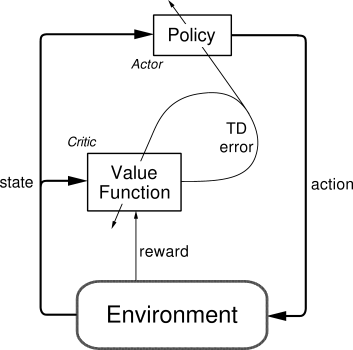
\includegraphics[width=35ex]{figures/figtmp34.png}\end{center}

\section{Entropie Maximierung}
Während standard RL Algorithmen nur die Belohnung maximieren, maximiert Soft Actor-Critic zusätzlich die Entropie der policy. Die Entropie ist höher, je ungenauer festzustellen ist, welche Aktion die optimale ist. Dies regt somit mehr zum Erforschen der Umgebung an. Die Entropie-Maximierung wird mit dem temperature-Wert $\alpha$ reguliert.

\begin{equation}
	\sum_{t=0}^T \mathbb{E}_{(s_t,a_t)\sim\rho_\pi}[{\mathnormal{r}(s_t,a_t)} + \alpha \mathcal{H}(\pi(\cdot|s_t))]
\end{equation}

Der temperature-Wert kann entweder initial gesetzt werden, oder über gradient descent gelernt werden. Zweiteres ist zu bevorzugen, da die Einstellung von $\alpha$ zur Laufzeit angepasst werden müsste, um sich der verändernden policy anzupassen. Das Lernverfahren erfolgt über folgende Fehlerfunktion:

\begin{equation}
J(\alpha)=\mathbb{E}_{a_{t}\sim\pi_{t}}\left[-\alpha \mathrm{log}\pi_{t}(a_{t}|s_{t})-\alpha \mathcal{H}\right]
\end{equation}

\section{Update Regeln der Netze}
Die Optimierung des Critic- und Actor-Netzwerkes erfolgt ebenfalls über gradient descent. Das Critic-Netzwerk versucht die folgende Fehlerfunktion zu minimieren:

\begin{equation}
J_{Q}(\theta)=
\end{equation}
\begin{equation}
\mathbb{E}_{(s_{t},a_{t})\sim D}\left[\frac{1}{2}(Q_{\theta}(s_{t},a_{t})-(r(s_{t},a_{t})+\gamma \mathbb{E}_{s_{t+1}\sim p}[V_{\overline{\theta}}(s_{t+1})]))^{2}\right]\notag
\end{equation}

Dabei ist

\begin{equation}
	\mathnormal{V}_{\overline{\theta}}(s_{t}) = \mathbb{E}_{a_t \sim \pi}[\mathnormal{Q}_{\overline{\theta}}(s_t, a_t) - \alpha \, \mathrm{log} \, \pi (a_t|s_t)]
\end{equation}

der value eines gegebenen Zustandes, mit Parametern $\overline{\theta}$ des target-Netzwerkes

Die Fehlerfunktion des Actors lautet:
\begin{equation}
J_{\pi}(\phi)=\mathbb{E}_{s_{t}\sim D}\left[\mathbb{E}_{a_{t}\sim \pi_{\phi}}\left[\alpha \mathrm{log}(\pi_{\phi}(a_{t}|s_{t}))-Q_{\theta}(s_{t},a_{t})\right]\right]
\end{equation}

\section{Reparameterization Trick}
Das Ziel des reparameterization tricks ist es, das stochastische Actor-Netzwerk durch Reparametrisierung in ein deterministisches umzuwandeln. Die geschieht über eine Abbildung auf den Aktionsraum, welcher über einen noise Vektor $\epsilon$ die Aktionen sampelt. Dadurch wird die Gradientenberechnung und somit das Training erleichtert.

\begin{equation}
a_{t}=f_{\phi}(\epsilon_{t};s_{t})
\end{equation}
Die Fehlerfunktion des Actors kann dann wie folgt umgeschrieben werden:

\begin{equation}
J_{\pi}(\phi)=\mathbb{E}_{s_{t}\sim D,\epsilon_{t}\sim N}\left[\alpha\mathrm{log}\pi_{\phi}(_{\phi}(\epsilon_{t};s_{t})|s_{t})-Q_{\theta}(s_{t},_{\phi}(\epsilon_{t};s_{t}))\right]
\end{equation}

\section{Algorithmus}

\begin{algorithm}[H]
        {\small
        \SetAlgoLined
        Input $\theta_{1}$,$\theta_{2}$ ,$\phi$\\
        $\overline{\theta_{1}} \leftarrow  \theta_{1}$ ,
        $\overline{\theta_{2}} \leftarrow \theta_{2}$ ,
        $\mathcal{D} \leftarrow \emptyset$\\
        \For{each iteration}{
             \For{each environment step}{
                  $a_{t}\sim \pi_{\phi}(a_{t}|s_{t})$,
                  $s_{t+1}\sim p(s_{t+1}|s_{t},a_{t})$\\
                  $D \leftarrow D \cup \{(s_{t},a_{t},r(s_{t},a_{t}),s_{t+1})\}$\\
             }
             \For{each gradient step}{
                $\theta_{i} \leftarrow \theta_{i}-\lambda_{Q}\hat{\nabla}_{\theta_{i}}J_{Q}(\theta_{i})$ for $i \in \{1,2\}$ \\
                $\phi \leftarrow \phi - \lambda_{\pi}\hat{\nabla}_{\phi}J_{\pi}(\phi)$\\
                $\alpha \leftarrow \alpha - \lambda\hat{\nabla}_{\alpha}J(\alpha)$\\
                $\overline{\theta_{i}} \leftarrow \tau\theta_{i} + (1-\tau)\overline{\theta_{i}}$ for $i \in \{1,2\}$ \\
            }
        }
        }
         \caption{Soft Actor-Critic}
\end{algorithm}

\end{multicols}




\end{document}